\documentclass[letterpaper,12pt,oneside]{book}
\usepackage[top=1in, left=0.9in, right=1.25in, bottom=1in]{geometry}
\usepackage{bachelorstitlepageUNAM}
\usepackage[utf8]{inputenc}
\usepackage[T1]{fontenc}
%\usepackage{biblatex}
%\addbibresource{biblatex-examples.bib}
\usepackage[backend=biber,style=apa]{biblatex}
\bibliography{Bibliografia.bib}
\usepackage[spanish,es-nodecimaldot,es-tabla]{babel}
\usepackage{graphicx}
\usepackage{tikz} 
\usepackage{tocloft}
\usepackage{amsmath}
\usepackage{blindtext}
\usepackage{longtable}
\usepackage{hyperref}
\hypersetup{
    colorlinks=true,
    linkcolor=blue,
    filecolor=magenta,      
    urlcolor=cyan,
    pdftitle={Overleaf Example},
    pdfpagemode=FullScreen,
   }
   \usepackage{multirow}%permite la modificacion de las tablas
   \usepackage{colortbl}
   \usepackage{float}
   \usepackage{amssymb, amsmath}
   \decimalpoint
   \usepackage{listings}
   \usepackage{amsfonts}
   \usepackage{bbm}
   \usepackage{bm}
   \usepackage{mathtools}
   \usepackage{matlab-prettifier}
   \usepackage{amsthm}
   \usepackage{titlesec}
   \usepackage{setspace}
   %\renewcommand{\baselinestretch}{2}
   %%% Definición de teoremas y lemas %%
   % https://es.overleaf.com/learn/latex/Theorems_and_proofs
   \newtheorem{theorem}{Teorema} 
   \newtheorem{proposition}[theorem]{Proposición}
   \newtheorem{lemma}[theorem]{Lema}
   \newtheorem{corollary}[theorem]{Corolario}
   

\title{Tesis de licenciatura Minerva} 
\author{Minerva Romero}

\IfFileExists{\jobname.run.xml}
{
%\includeonly{
%  introduccion,
%  material_metodo,
%  resultados,
%  discusion,
%  append
%  }
}
{
% Compile inicialmente el documento completo para generar
% todos los ficheros .aux
}

\begin{document}
\frontmatter

%------------------------------

\begin{titlepage}
    \thispagestyle{empty}
    \begin{minipage}[c][0.17\textheight][c]{0.25\textwidth}
        \begin{center}
            
\includegraphics[width=3.5cm, height=3.5cm]{Escudo-UNAM.pdf}
        \end{center}
    \end{minipage}
    \begin{minipage}[c][0.195\textheight][t]{0.75\textwidth}
        \begin{center}
            \vspace{0.3cm}
            \textsc{\large Universidad Nacional Aut\'onoma de M\'exico}\\[0.5cm]
            \vspace{0.3cm}
            \hrule height2.5pt
            \vspace{.2cm}
            \hrule height1pt
            \vspace{.8cm}
            \textsc{Facultad de Ciencias}\\[0.5cm] %
        \end{center}
    \end{minipage}

    \begin{minipage}[c][0.81\textheight][t]{0.25\textwidth}
        \vspace*{5mm}
        \begin{center}
            \hskip2.0mm
            \vrule width1pt height13cm 
            \vspace{5mm}
            \hskip2pt
            \vrule width2.5pt height13cm
            \hskip2mm
            \vrule width1pt height13cm \\
            \vspace{5mm}
            
\includegraphics[height=4.0cm]{Escudo-FCIENCIAS.pdf}
        \end{center}
    \end{minipage}
    \begin{minipage}[c][0.81\textheight][t]{0.75\textwidth}
        \begin{center}
            \vspace{1cm}

            {\large\scshape Análisis de la cienciometría en biociencias}\\[.2in]

            \vspace{2cm}            

            \textsc{\LARGE T\hspace{1.5cm}E\hspace{1.5cm}S\hspace{1.5cm}I\hspace{1.5cm}S}\\[0.5cm]
            \textsc{\large que para obtener el t\'itulo de:}\\[0.5cm]
            \textsc{\large Matemáticas Aplicadas}\\[0.5cm]
            \textsc{\large presenta:}\\[0.5cm]
            \textsc{\large {Minerva María Romero Pérez}}\\[2cm]          

            \vspace{0.5cm}

            {\large\scshape Tutora:\\[0.3cm] {Dra. Layla Michán Aguirre }}\\[.2in]

            \vspace{0.5cm}

            \large{Ciudad Universitaria,Ciudad de México}{ }{2024}
        \end{center}
    \end{minipage}
\end{titlepage}

%---------------------------------

% =========================
\mainmatter
\tableofcontents
\documentclass[../Main.tex]{subfiles}
%%%%------------Introducción------------%%%%%%
\begin{document}
\noindent
La información es una fuente importante para hacer investigación se \parencite{hull_defrosting_2008}\\ 
Las biociencias son …
\smallskip
Los análisis métricos de las publicaciones científicas ha crecido junto con la tecnología informática e informacional en la Web…

\smallskip
Entre métodos más usados para realizar los análisis están: la minería de textos, la ciencia de datos, los análisis de redes, los análisis métricos y los grandes datos…

\smallskip
instituciones e investigadores que utilicen la cienciometría… 

\smallskip
Actualmente, existen instituciones como el Centre for Science and Technology Studies (CWTS) traducido al español como Centro de Estudios de Ciencia y Tecnología, en el cual con la bibliometría y la cienciometría estudian la investigación científica (\url{https://www.cwts.nl/about-cwts}) …
\smallskip
Silvio Peroni... 
Ludo Wltman… 
Daniel Torres Salinas … 
La ciencia abierta es un …
\section{Lenguaje natural y lenguaje máquina}
\noindent
El lenguaje natural es la forma en la que las personas hablamos y vemos la información, esta es la que entendemos y es como visualizamos comúnmente las cosas en la web. Mientras que el lenguaje máquina es estructurado, interoperable y no es comprensible a simple vista, es leído por computadoras y es como funcionan los programas y la web. 

\section{Los metadatos}
\noindent
Los metadatos son comúnmente conocidos como los datos sobre los datos. Estos constituyen Información estructurada que describe, explica, localiza y hace que sea más fácil de recuperar, utilizar o manejar la información (NISO,XX). Estos pueden ser estructurales, descriptivos o administrativos. Los estructurales son …\parencite{gartner_metadata_2016}\parencite{pomerantz_metadata_2015}


\smallskip
El uso de metadatos adecuados permiten una correcta estructuración y descripción de los datos, puesto que detallan las características de la información que se genera, como la fecha de creación, la licencia de uso, el autor, el tipo de objeto digital (texto, imagen, sonido, video) o la dirección electrónica en la que se encuentra alojado.

\smallskip
Los metadatos bibliográficos son útiles para el fácil procesamiento de la información, ayudan al estudio de las publicaciones científicas, con ellos se pueden generar análisis para ver patrones y responder preguntas científicas sobre las investigaciones. Este tipo de metadatos se originan a partir de la información proporcionada por los autores, revistas y bases de datos bibliográficas.

\smallskip
Cada revista científica tiene una fecha de publicación de sus números, lo que genera los metadatos de fecha de publicación, las bases de datos generan los metadatos de cuando reciben y agregan las publicaciones, entonces se van generando distintos metadatos con fechas, para realizar una revisión de literatura y tomar el conjunto de publicaciones se tienen que tener en consideración estas, ya que hay que tener muy bien definido el intervalo de tiempo del que se van a obtener los textos.

\smallskip
La diferencia entre la lectura natural y la lectura máquina de los metadatos se muestra en la figura 1, en la cual se puede ver que el lenguaje natural es como encontramos comúnmente la información de la Web, mientras que el lenguaje máquina muy pocos lo conocen, pero es la forma en la que se maneja la información para su análisis, manejo y procesamiento. 

\smallskip  
Formato RIS son las siglas de la empresa que lo desarrollo Research Information Systems, en español Sistemas de información de investigación, es un formato de etiquetado en el cual se separan los metadatos, se agrega la etiqueta espacio, guion, espacio y el metadato asociado a la etiqueta. Se utiliza para el intercambio de información de citas. Por ejemplo, los gestores bibliográficos aceptan este formato para manejar las citas, y las bases de datos bibliográficas manejan este para tener los metadatos y poder exportarlos.
%%%%%%%%%%%%%%%%%%%%%%falta completar 

\section{Las bases de datos bibliográficas}
\noindent
Las bases de datos son fuentes en las cuales permiten procesar, guardar, ordenar, mantener y presentar datos. Son sistematizadas, presentan la información en tablas con un orden establecido, por lo que se tiene mucha información en poco espacio. Las bases de datos permiten realizar búsquedas a partir de distintos criterios, procesar datos de forma cuantitativa y cualitativa, interrelacionar los resultados utilizando distintas variables y actualizar la información fácil y rápidamente.

\smallskip
Las bases de datos se extienden por módulos y se pueden diseñar, almacenar, manejar y analizar en una computadora, son compatibles con otras bases de datos, en estas se pueden hacer consultas (‘queries’) para realizar cálculos, las bases de datos relacionales son las más utilizadas, presentan los datos en dos o más tablas (constituidas por registros o renglones y columnas) que están relacionadas entre sí por medio de la repetición de un atributo.
Las bases de datos pueden ser estáticas en donde la información no varía en el tiempo o dinámicas las cuales se actualiza, cambia o elimina la información después de algún tiempo. 

\smallskip
Las bases de datos biológicas son una herramienta indispensable para el quehacer de los biólogos, estas permiten… 

\smallskip
Las bases de datos bibliográficas se encargan de manejar información estructurada, sobre los artículos, libros, capítulos o memorias. Las bases de datos bibliográficas manejan los metadatos dados por los autores y revistas, algunas agrega metadatos como identificadores, ontologías y tesauros.  

\smallskip
Existen muchas bases de datos bibliográficas, desde especializadas en áreas como la medicina, que solo contienen artículos o solo libros y hay multidisciplinarias y que contienen cualquier tipo de publicación como artículos, preprints, libros, patentes, etc. Entonces es importante saber qué información contienen y que información necesitamos para elegir la o las más relevantes para trabajar. Entre las características más importantes a considerar están: criterios de inclusión de documentos, contenido (tipo de registros), tipo de acceso, la cobertura (representación) tipológica, temática, geográfica y temporal de la colección
Dentro de las bases de datos biológicas se encuentran las bases de datos bibliográficas sobre biociencia estas resultan utiles para generar nuevo conocimiento\\
Entonces algo fundamental en la Web son los datos ligados estos nos permiten tener la información conectada desde diferentes enfoques … 

\smallskip
Indexar es  agregar a un catálogo cualquier tipo de información, por ejemplo revistas, artículos, términos estructurados, etc. Entonces se tiene que las bases de datos bibliográficas indexan revistas de acuerdo a ciertos criterios que implementa la base de datos. 
    
\section{PubMed}
\noindent
Una de las bases de datos bibliográficas más importantes para la medicina es PubMed, unas de sus características más importantes es que es de exceso abierto, es amigable y tienen una gran cantidad de herramientas, estas características y más pueden consultarse en … (articulo herramientas de pubmed texto ,\url{https://zenodo.org/records/10659207}). 
Para este trabajo es de interés el tesauro MeSH asociado a PubMed este es un vocabulario controlado ... 

\section{Las APIs}
\noindent
Una API o Interfaz de Programación de Aplicaciones (por sus siglas en inglés, Application Programming Interface), es un conjunto de reglas y protocolos que permiten que diferentes aplicaciones o sistemas informáticos se comuniquen entre sí.
Estas definen los métodos y datos que las aplicaciones pueden utilizar para interactuar unas con otras de manera estandarizada y predecible

\smallskip
Las APIs son esenciales para la integración y la interoperabilidad entre sistemas de software, y se utilizan en una variedad de contextos, incluyendo aplicaciones web, aplicaciones móviles, sistemas operativos, bases de datos, servicios en la nube y más. Algunos de los conceptos clave relacionados con las APIs son:  

 \smallskip
\begin{itemize}
\item Estándares y protocolos: para garantizar la consistencia y la compatibilidad.
\item Interfaz de usuario vs. interfaz de programación: en donde la interfaz de usuario permite que las personas interactúen con la aplicación, mientras que la API o interfaz de programación permite que los programas y sistemas interactúen entre sí sin necesidad de intervención humana
\item Datos estructurados: las APIs suelen transmitir datos en un formato estructurado, esto puede ser en formato JASON (JavaScript Object Notation) o XML (eXtensible Markup Language) y facilitan la interpretación y el procesamiento de la información por parte de las aplicaciones
\item Seguridad: las APIs pueden requerir autenticación y autorización para garantizar que solo las aplicaciones autorizadas puedan acceder a sus servicios. Esto es fundamental para proteger la privacidad y la seguridad de los datos.
\item Documentación: Las buenas APIs suelen estar acompañadas de documentación detallada que describe cómo utilizarlas, qué métodos están disponibles y qué datos se pueden esperar en las respuestas.
\end{itemize}

Las APIs son utilizadas en una amplia gama de aplicaciones, desde la integración de servicios de terceros en aplicaciones móviles hasta la automatización de tareas en sistemas empresariales. Permiten a los desarrolladores aprovechar las funcionalidades de otros sistemas de manera eficiente, lo que acelera el desarrollo de software y la creación de aplicaciones más poderosas y versátiles. 

 \smallskip
En este trabajo nos interesa explorar las APIs de bases de datos bibliográficas, ya que estas son las que nos van a permitir extraer metadatos de las publicaciones de una manera eficiente y rápida para poder realizar análisis de la información  

\smallskip
Adicionalmente, PubMed se tiene disponible la API (Application Programming Interface) que sea la cual define los métodos y datos que las aplicaciones pueden utilizar para interactuar con la base de datos unas con otras de manera estandarizada y predecible, para lo que permite para exportar registros y para procesarlos por métodos informáticos que implican programación y conocimiento en el funcionamiento de las aplicaciones. Además, hay una buena documentación disponible con los detalles técnicos, lo que promueve que incluso los usuarios puedan crear aplicaciones. 

\section{Revisiones de literatura}
\noindent
Una revisión de literatura es … 

\smallskip
Existen distintos tipos de revisiones de literatura, en   capitulo biorevisiones de literatura, X se pueden ver algunas con sus ejemplos y..

\section{La cienciometría}
\noindent
La cienciometría puede considerarse un tipo de revisión de literatura ( capitulo biorevisiones de literatura,X) 

 \smallskip
Para realizar análisis cienciométricos existen aplicaciones web y software para computadora desde los cuales se puede procesar los datos, algunas de estas herramientas son amigables pero, algunas no …(XX) 

\smallskip
La ciencimetría abierta es …, las ventajas de esta son (XX)  

\section{Leyes e indicadores cienciometrícos}
\noindent
Cuando se hace un análisis bibliométrico se utilizan las tres leyes de la bibliometría y los indicadores cienciométricos, las cuales …  

\subsection{Ley de Lotka}
\noindent
La proporción de autores que han publicado $n$ artículos dentro de un campo científico es inversamente proporcional al cuadrado de $n$. De lo cual obtenemos lo siguiente (Urbizagástegui Alvarado, 1999):
$$A(n)=\frac{C_1}{n^2}$$
De donde: 
$A(n):$ es la función que indica la fracción de autores que han publicado $n$ artículos 
$C_1:$ es el número de publicaciones por cada autor  
$n:$ el número de publicaciones dentro de un campo científico  
\subsection{Ley de branford }
\noindent
\subsection{Ley de Zipf}
\noindent

\section{Cienciometría para ciencias de la vida y de la salud}
\noindent
La cienciometría es  

\section{Análisis de redes}
\noindent
Para entender la definición de red es necesario dar una introducción a la teoría de gráficas.\\
Una gráfica es un conjunto $(X,A)$ donde $X$ es el conjunto no vacío de elementos llamados nodos o vértices, y $A$ es el conjunto de pares no ordenados de vértices o nodos que llamados aristas o vértices.\\
Una gráfica puede ser dirigida o no, le llamamos dirigida a las que cumplen que  \\

Una red es una gráfica dirigida en la cual se le asocia una función $f$ a los arcos, nodos o ambos \parencite{hernandez_redes}. En general, el término red se refiere a problemas reales como redes metabólicas, redes de cooperación en artículos o redes de documentos web \parencite{barabasi_network_2016}.

\section{Objetivos}
\noindent
El objetivo de mi investigación es analizar la bibliografía en Biociencias para entender cómo se ha usado la cienciometría, y otros métodos métricos relacionados, como la bibliometría, la infometría y la altmetría, en la literatura sobre el COVID-19 en los tres enfoques que son la enfermedad, la pandemia y el virus, en los cuales se ha contribuido en nuevo conocimiento.  
Además, quiero reunir las herramientas informáticas, los procesos y los protocolos informacionales e informáticos implementados en los análisis métricos para seleccionar los casos más relevantes y la tecnología de vanguardia, como, los grandes datos, el análisis de redes, la semántica, las ontologías, los datos ligados, algoritmos e inteligencia artificial.  
Este proyecto es multi, intra, trans e interdisciplinario, es original, inédito e integrativo, porque generalmente los análisis bibliométricos estudian un tema científico específico, pero en este caso tengo como objetivo principal estudiar los artículos cienciométricos publicados en biociencias, esto es, haré cienciometría de la cienciometría en ciencias de la vida y de la salud para sistematizarla y sintetizarla con los siguientes propósitos: 
\begin{itemize}
    \item Entender las diferentes formas en las que se ha utilizado la cienciometría para el COVID-19.
    \item Explorar y explicar las ventajas de hacer cienciometría abierta.
    \item Reunir y explorar las herramientas digitales amigables  y de código disponibles para realizar análisis de literatura y los métodos informáticos más útiles e innovadoras para PubMed.
    \item Descubrir la mejor manera de integrar, representar y contextualizar la información por medio de las visualizaciones.
    \item Reunir todos los análisis realizados para México.
    \item Realizar analisis de redes para ver las tendencias y patrones de los datos.
    \item Probar y estudiar las leyes de la blibliometría para analizar artículos. 
\end{itemize}





\end{document}
%%%%%%%%%%%%%%%%%%%%%%%%%%%%%%%%%%%%%%%%%%%%%%%%%%%%%%%%%%%%%%%
\chapter{Material y Método}
%\addcontentsline{toc}{chapter}{Material y Método}
\spacing{1.5}
Esta investigación \textit{in silico} centrada en el uso de recursos informáticos, 
basada en la literatura y sustentada en teorías matemáticas sobre los analisis cienciometrícos de COVID-19, 
constó de XXX etapas:  (figura XX) \\
%%%%%----diagrama 
\smallskip
Estas XX etapas son la base para realizar un analisis de cualquier tipo de literatura y en cualquier area de estudio. 
Durante estas etapas utilicé la base de dato bibliográfica PubMed y 
distintas herramientas digitales para la recuperación de la literatura, el procesamiento de la información, 
el análisis y la visualización de los datos.  
Hice uso del lenguaje de programación R en Rstudio, con las paqueterías, bibliometrix y ggplot2 
en una computadora Asus VivoBook con sistema operativo de 64 bits, procesador AMD Ryzen 7 4700U y RAM de 16.0 GB, 
esto me permitió realizar un análisis de la literatura de forma eficiente, rápida y estructurada,
además de poder visualizar los datos de una forma amigable y entendible.

%%%%%%
\section{Planeación}
\noindent
Además, entender el mundo de los análisis de literatura y las bases de datos bibliográficas, 
revise artículos, publicaciones, entrevistas y vídeos de expertos. El análisis cienciométrico 
es un proceso largo, generalmente realizada por equipos multidisciplinarios, que involucra una 
gran cantidad de datos, y que ha tenido un impulso a partir de la era de la digitalización, 
ya que resulta más sencillo tener acceso a las bases de datos de las cuales se extrae la información.

\section{Recuperación de la literatura en bases de datos}
\noindent
Para recuperar la literatura de una forma eficiente, 
use las APIs (Application Programming Interface) de las fuentes, 
para poder usaras, exploré su funcionamiento en distintos recursos como textos, 
plataformas, videos, etc.
Para esta etapa con ayuda del esquema de la Figura 2 organice los elementos para hacer una recuperación de literatura,  (ri biocolores 2023)
Utilice la base de datos bibliográfica PubMed, la cual es una de las bases de datos más grandes y 
completas de literatura científica y biomédica. Además use las herramienta asociadas a esta base de datos,
como la API de PubMed, para poder recuperar la literatura de una forma eficiente y rápida. La lista de estas 
herramientas se encuentra en la tabla (tabla).

\smallskip
Las biociencias son un campo de estudio muy amplio y por ende intentar buscar literatura de todo este sería una tarea titánica, 
es por esto que realice una primera busqueda, esta fue genraral para ver todas las publicaciones sobre cienciometría en PubMed 
en esta búsqueda utilice términos generales para mostrar y visualizar la gran cantidad de publicaciones que existen. 
La consulta utilizada fue evolucionando hasta obtener una consulta interesante que muestra los articulos que realizan análisis
de la información como articulos, redes sociales, tecnologías y documentos y que estuduan comportamientos en dos tipos de entidades 
la entidad salud como enfemedades, medicamentos, tratamientos y la entidad evaluativa como instituciones, investigadores, revistas, 
y hospitales\\
\framebox{\textbf{Consulta 0:} scientometric* OR bibliometr* OR altmetr* OR cybermetr* OR infometr*}

\smallskip
Ya que se obtuvo un conjunto muy grande de datos se tenia que acotar esta información, para esto en los resultados de la consulta 0
encontre que este tipo de revisiones tuvieron un gran aumento durante la pandemia de COVID-19 ya que hacer investigación desde un laboratorio
 fue complicado es por esto que los análisis de la información aumentaron (CITA).
 Entonces me parece interesante comocer cuantas de las publicaciones que hacen revisiones son del
 tema de COVID-19, encontrar las nuevas tecnologías y métodos innovadores desde
 distinto enfoques como lo son la enfermedad, la pandemia y el virus de estos tres años que han pasado desde el inicio de la pandemia.
 Y a pesar de que también hay documentos que fueron publicados en el periodo de la pandemia estas no las consideré, 
 puesto que no hablan propiamente del COVID-19.

\smallskip
Para el tema de COVID-19 realice distintas consultas en PubMed, susando los terminos MeSH operadores booleanos y 
operadores de truncamiento. En el siguiente cuandro se encunetra la consulta 1 que es una de las consultas que realice 
para obtener la consulta 2 que es la consulta final que utilice para extraer la información.\\

\noindent
\fbox{
\begin{minipage}[c][1.2\height]%
[c]{1\textwidth} \textbf{Consulta 1:} (Scientometr* OR Bibliometr* OR Altmetr* OR Cybermetr* OR Infometr* OR entitymetr*)AND (covid-19 OR SARS-CoV-2)\\
\textbf{Consulta 2:} (("Bibliometrics"[Mesh] OR entitymetr* OR scientometr* OR Altmetr* OR Cybermetr* OR Infometr* OR "metrics") AND ("COVID-19"[Mesh] OR "SARS-CoV-2"[Mesh])) NOT "Journal Impact Factor"[Mesh]
\end{minipage}}

\section{Definición de criterios de inclusión, de exclusión y las variables}
\noindent
Los artículos que incluí para la etapa dos tenían que cumplir con los siguientes criterios:
\begin{itemize}
    \item Tener el identificador DOI.
    \item Tener el identificador PMID.
    \item Ser sobre el virus, la enfermedad o la pandemia del COVID-19 o SARS-CoV-2.
    \item Artículos publicados entre el 2020 y 2023.
    \item No ser documentos que fueran publicados en el periodo de la pandemia del COVID-19
    \item Realiza un análisis cienciométrico explícitamente.
    \item No ser de factor de impacto, es decir, de la entidad evaluativa.
\end{itemize}
\subsection{Metadatos bibliográficos}
Los metadatos asociados a las publicaciones tienen un ciclo por el que se le va asociando los metadatos, 
primero la revista le pide al autor ingresar datos como titulo, 
resumen, palabras clave y autores, segundo la revista al publicar genera metadatos como el DOI 
y otros identificadores, tercero las bases de datos cuando indexan los documentos generan 
metadatos como identificadores (PMID), cuarto los usuarios pueden generar nuevos metadatos obteniéndolos 
desde el documento para poder realizar análisis más robustos (Figura).%%%% Hacer un diagrama de el ciclo de los metadatos
Los metadatos son información que se evalúa en un análisis de la literatura, 
es por esto que se usan como variables, utilice tanto metadatos generados por la revista los autores, 
los que generé y los que se pueden obtener de la base de datos PubMed.  
En la tabla \ref{tab:variables} se muestra en la columna cuatro, 
origen de los metadatos, la etapa en la cual se originó cada metadato 
extraído. 
Durante el procedimiento registré todas las variables factibles 
para ser analizadas (Tabla \ref{tab:variables}) y  después seleccioné las variables 
que usé para las siguientes etapas.  
%%%%% Cambiar la tabla%%%%%
%%% Poner la tabla en vertical para que quede en una hoja 
\begin{longtable}{|p{2cm}|p{2cm}|p{2cm}|p{1.2cm}|p{1.9cm}|p{1.5cm}|p{2.1cm}|}
\hline
\textbf{Nombre}   & \textbf{Categoría}         & \textbf{Descripción de la categoría}     & \textbf{Origen}& \textbf{De que}  & \textbf{asociado}& \textbf{URL}                                        \\
                  & \textbf{}                  & \textbf{}                                & \textbf{     } & \textbf{es}      & \textbf{a}      & \textbf{}                                           \\ \hline
Enfermedad        & Objeto de estudio COVID    & Enfoque del estudio sobre COVID 19       &                & Estudio          &                &                                                     \\ \hline
Pandemia          & Objeto de estudio COVID    & Enfoque del estudio sobre COVID 19       &                & Estudio          &                &                                                     \\ \hline
Virus             & Objeto de estudio COVID    & Enfoque del estudio sobre COVID 19       &                & Estudio          &                &                                                     \\ \hline
Artículos         & Tipo de información        & Tipo de información estudiad             & Yo             & Estudio          &                &                                                     \\ \hline
                  & Cantidad de registros      & \# de registros utilizados en el estudio & Yo             & Estudio          &                &                                                     \\ \hline
                  & Fecha de inicio            & Fechas de inicio del estudio             & Yo             & Estudio          &                &                                                     \\ \hline
                  & Fecha de fin               & Fechas de fin del estudio                & Yo             & Estudio          &                &                                                     \\ \hline
                  & Intervalo de tiempo        & Intervalo de tiempo del estudio          & Yo             & Estudio          &                &                                                     \\ \hline
                  & Consulta                   & Consulta realizada en el estudio         & Yo             & Estudio          &                &                                                     \\ \hline
                  & Software                   & Software utilizado en el estudio         & Yo             & Estudio          &                &                                                     \\ \hline
                  & API´s                      & API's utilizadas                         & Yo             & Estudio          &                &                                                     \\ \hline
                  & Tipo de estadísticas       & Tipo de estadísticas                     & Yo             & Estudio          &                &                                                     \\ \hline
                  & Enfermedad                 & Enfermedad asociada al COVID 19          &                & Estudio          &                &                                                     \\ \hline
Cienciometría     & Tipo de análisis           & Tipo de análisis métrico realizado       & Yo             & Estudio          &                &                                                     \\ \hline
Bibliometría      & Tipo de análisis           & Tipo de análisis métrico realizado       & Yo             & Estudio          &                &                                                     \\ \hline
IA                & Tipo de tecnologías        & Tipos de tecnologías usadas              & Yo             & Estudio          &                &                                                     \\ \hline
Mineria de textos & Tipo de tecnologías        & Tipos de tecnologías usadas              & Yo             & Estudio          &                &                                                     \\ \hline
Análisis de redes & Tipo de tecnologías        & Tipos de tecnologías usadas              & Yo             & Estudio          &                &                                                     \\ \hline
PubMed            & Base de datos              & Que DB se utilizó en el estudio          & Yo             & Estudio          &                &                                                     \\ \hline
                  & Otras DB asociadas         & Otras DB utilizadas durante el estudio   & Yo             & Estudio          &                &                                                     \\ \hline
                  & Herramientas digitales     & Herramientas utilizadas en el estudio    & Yo             & Estudio          &                &                                                     \\ \hline
Journal Article   & Tipo de documento          & Tipo de documento decuerdo con MeSH      & DB             & Documento        & MeSH           & \url{https://meshb-prev.nlm.nih.gov/record/ui?ui=D016428} \\ \hline
Review            & Tipo de documento          & Tipo de documento decuerdo con MeSH      & DB             & Documento        & MeSH           & \url{https://meshb-prev.nlm.nih.gov/record/ui?ui=D016454} \\ \hline
Abierto           & Tipo de acceso             & Tipo de acceso al documento              &                & Documento        &                &                                                     \\ \hline
DOI               & Identificador              & identificador asociado al documento      & Revista        & Documento        &                &                                                     \\ \hline
PMID              & Identificador              & identificador asociado al documento      & DB             & Documento        &                &                                                     \\ \hline
PMCID             & Identificador              & identificador asociado al documento      & DB             & Documento        &                &                                                     \\ \hline
                  & Citas                      &                                          &                & Documento        &                &                                                     \\ \hline
    *             & Palabras clave             &                                          &                & Documento        &                &                                                     \\ \hline
    *             & Terminos MeSH              &                                          & DB             & Documento        &                &                                                     \\ \hline
    *             & Autores                    &                                          &                & Documento        &                &                                                     \\ \hline
                  & Adscripción de los autores &                                          &                & Documento        &                &                                                     \\ \hline
                  & Título                     &                                          &                & Documento        &                &                                                     \\ \hline
                  & Resumen                    &                                          &                & Documento        &                &                                                     \\ \hline
                  & Fecha de publicación       &                                          &                & Documento        &                &                                                     \\ \hline
    *             & Revista                    &                                          &                & Documento        &                &                                                     \\ \hline
                  & Idioma                     &                                          &                & Documento        &                &                                                     \\ \hline
\caption{\textit{Tabla con las variables que se pueden evaluar de estas, solo seleccione las que se encuentran con *.}}
\label{tab:variables}
\end{longtable}
Las variables que serán usadas se eligieron para poder ver las leyes de la bibliometría y para hacer análisis de redes.
\begin{itemize}
    \item Los autores son las personas que contribuyeron para la realización de la publicación, 
    cada investigador tiene un área de especialidad.
    \item Las revistas son  publicaciones periódicas que tienen un enfoque y alcance específico, 
    en las que se publican los textos revisados por pares que cumplen con los requisitos de la revista. 
    \item Las palabras clave de un texto son uno o más términos en los cuales se describe la investigación. 
    Estas son metadatos básicos de cualquier texto y son generados por los autores al publicar en una revista.  
    \item Los términos MeSH son términos estandarizados del tesauro MeSH, estos se utilizan para indexar, 
    catalogar y buscar información biomédica y relacionada con la salud. Estos términos en PubMed se pueden ver y 
    descargar como metadatos asociados a los textos \parencite{noauthor_medical_2023}.
\end{itemize}

\section{Extracción de los datos}
\noindent
Primero realice un analisis rapido de los datos con ayuda de la herramienta PubReMiner, 
posterirmente para obtener los datos necesarios para el análisis de manera eficiente y rápida extraje 
los metadatos mediante la API de PubMed,
%%%Ver porque desde la API obtengo un resultado diferente al de la plataforma y explicar aquí


\section{Procesamiento de la información de la literatura}
\noindent
la
\section{Análisis}
\noindent
Dos grandes formas en las cuales se pueden procesar metadatos biométricamente son desde 
aplicaciones en línea amigables, las cuales muchas veces están asociadas a bases de datos y 
 software en los que se necesita conocimiento en programación y resultan no ser amigables.\\
Ejemplos\\
Para realizar el análisis utilicé Bibliometrix una paquetería de R \parencite{bibliometrix}

\section{Visualización de datos}
\noindent
de
\section{Integración y contextualización de la información}
\noindent
Durante la

\smallskip
Para el registro de los artículos y notas, utilice hypothes.is. Una herramienta digital de gran 
utilidad que nos parece muy valiosa para la investigación digital.

\smallskip
Para mantenerme actualizada de nuevas publicaciones de los distintos temas en biociencias, genere los RSS
%%%%%%%%%%%%%%%%%%%%%%%%%%%%%%%%%%%%%%%%%%%%%%%%%%%%%%%%%%%%%%%
\chapter{Resultados}
%\addcontentsline{toc}{chapter}{Resultados} % Añadir a la tabla de contenidos si es que no aparece
\spacing{1.5}

De la consulta 0 obtuve 18,825 resultados, de los cuales podemos ver la cantidad de publicaciones que hay al año y se muestran en la Figura \ref{fig:consulta0} en la cual se puede ver que a partir del 2020 aumentaron drásticamente las publicaciones sobre cienciometría, bibliometría, y los análisis de la literatura. 
\begin{figure}[H]
\centering
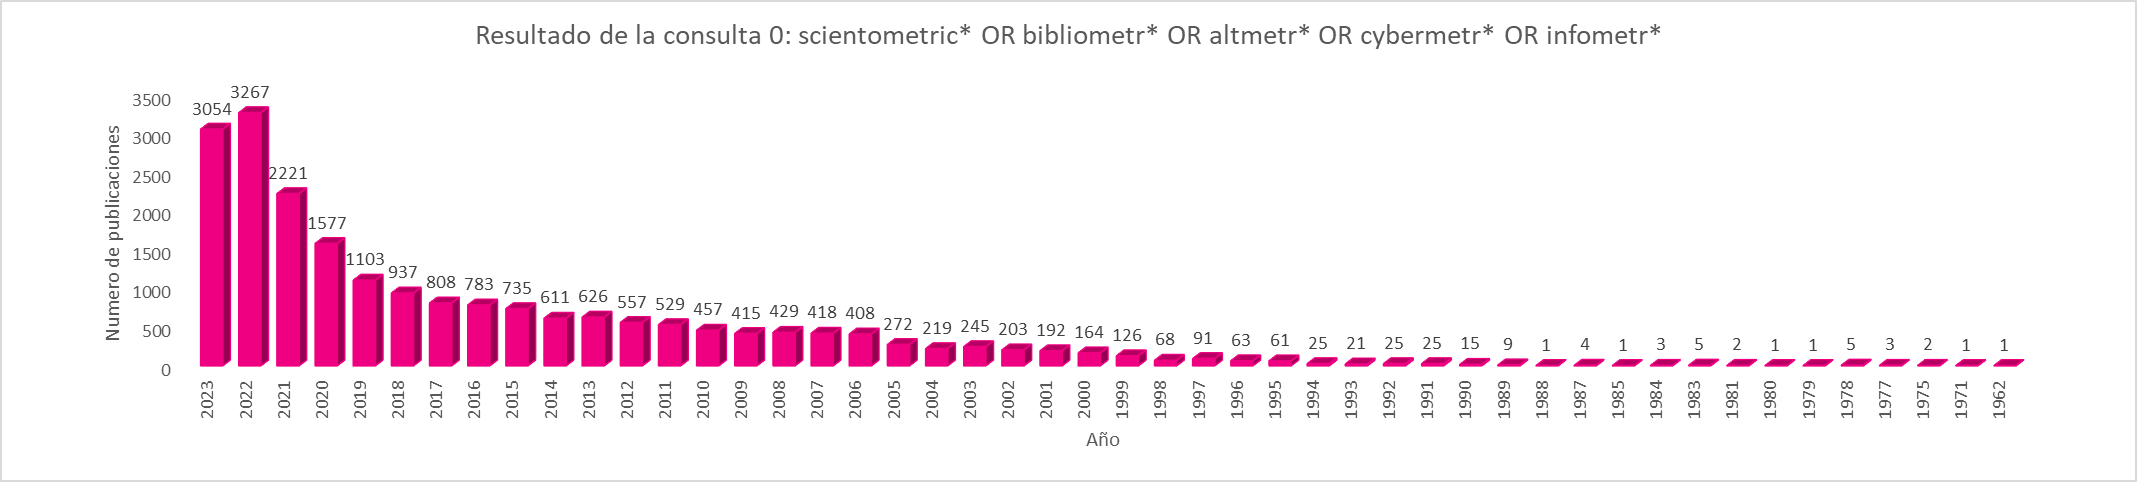
\includegraphics[width=1\textwidth]{Imagenes/consulta0.png}
\caption{\textit{Gráfica de la cantidad de publicaciones por año de la consulta 0}}
\label{fig:consulta0}
\end{figure}
De la consulta 1 obtuve 1,011 resultados de los cuales...\\
De la consulta 2 obtuve 1,784 resultados de los cuales...\\
\documentclass[../Main.tex]{subfiles}

\begin{document}
\noindent
%%%%------------Discusión/conclusión ------------%%%%%%
De esta manera se tienen los desdoblamientos hiperfinos, los cuales se muestran en la 

\end{document}
\appendix
%%%%%%%%%%%%%%%%%%%%%%%%%%%%%%%%%%%%%%%%%%%%%%%%%%%%%%%%%%%%%%%
\chapter{Apéndice}
\spacing{1.5}
El contenido del primer apéndice.

% ========================
\backmatter
\printbibliography
\end{document}

%%%%%%%%%%%%%%%%%%%%%%%%%%%%%%%%%%%%%%%%%%%%%%%%%%%%%%%%%%%%%%%